\section{Exemples d'images RETIF}

\begin{figure}[H]
    \centering
    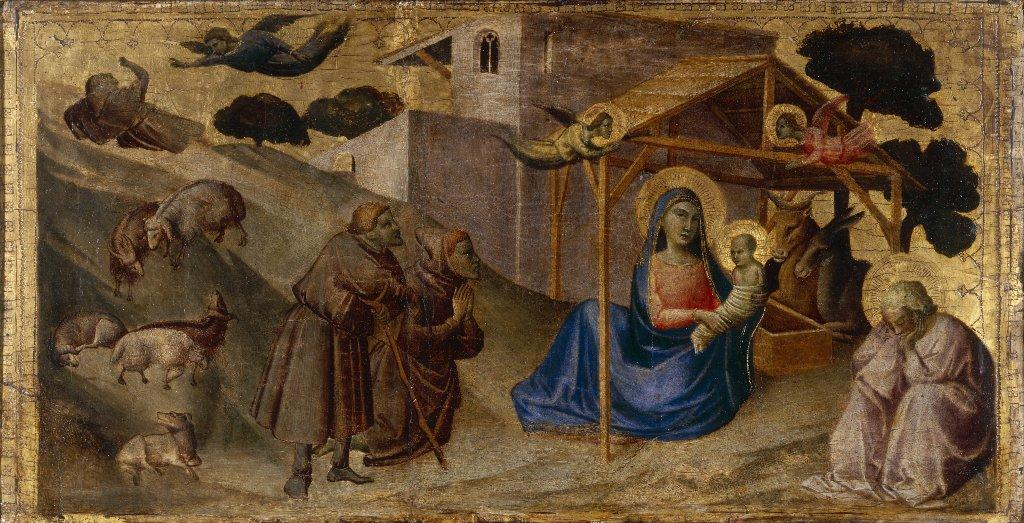
\includegraphics[width=0.7\textwidth]{annexes/figures/ptrGaddiAdoration.jpg}
    \caption{Taddeo Gaddi, \textit{L'Adoration des bergers}, vers 1330, tempéra sur bois, Dijon, Musée des Beaux-Arts, inv. 1470 © Musée des Beaux-Arts de Dijon}
    \label{fig:ptrGaddiAdoration}
\end{figure}


\begin{figure}[H]
    \centering
    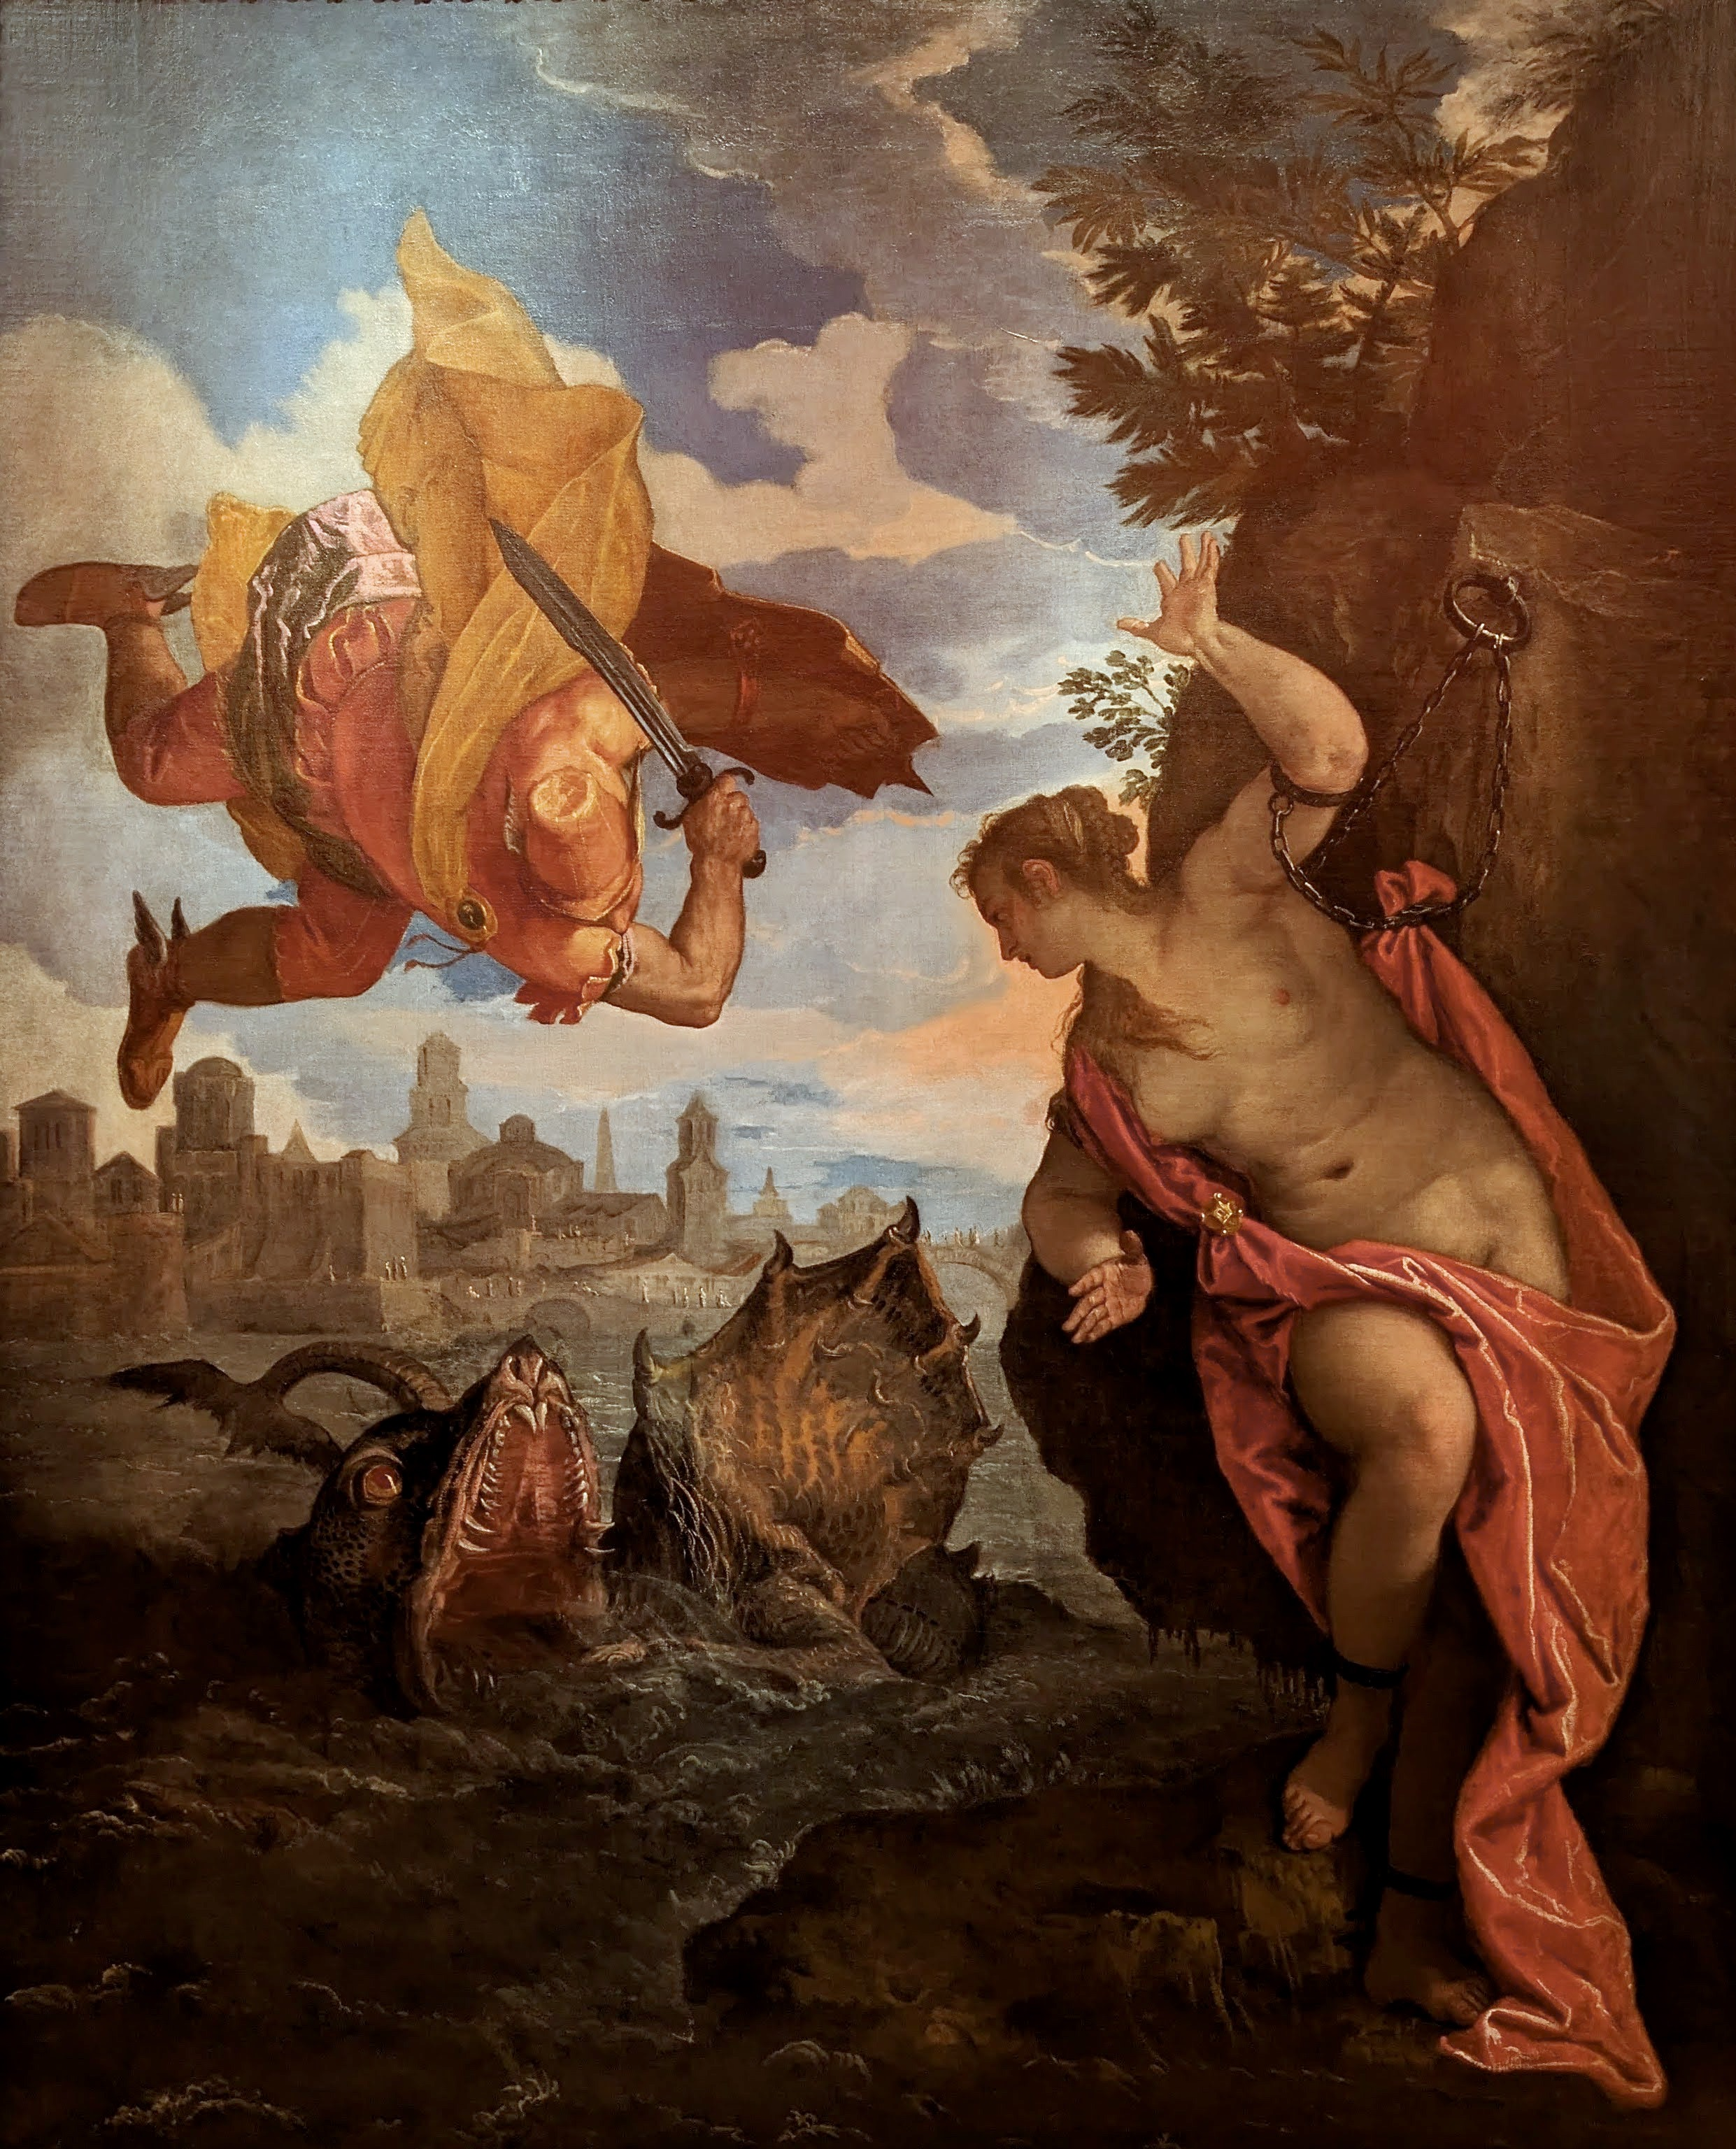
\includegraphics[height=0.4\textheight]{annexes/figures/ptrVeronesePersee.jpg}
    \caption{Paul Véronèse, \textit{Persée délivrant Andromède}, 1575-1580, peinture à l'huile sur toile, Rennes, Musée des Beaux-Arts de Rennes, inv. 801.1.1}
    \label{fig:ptrVeronesePersee}
\end{figure}

\begin{figure}[H]
    \centering
    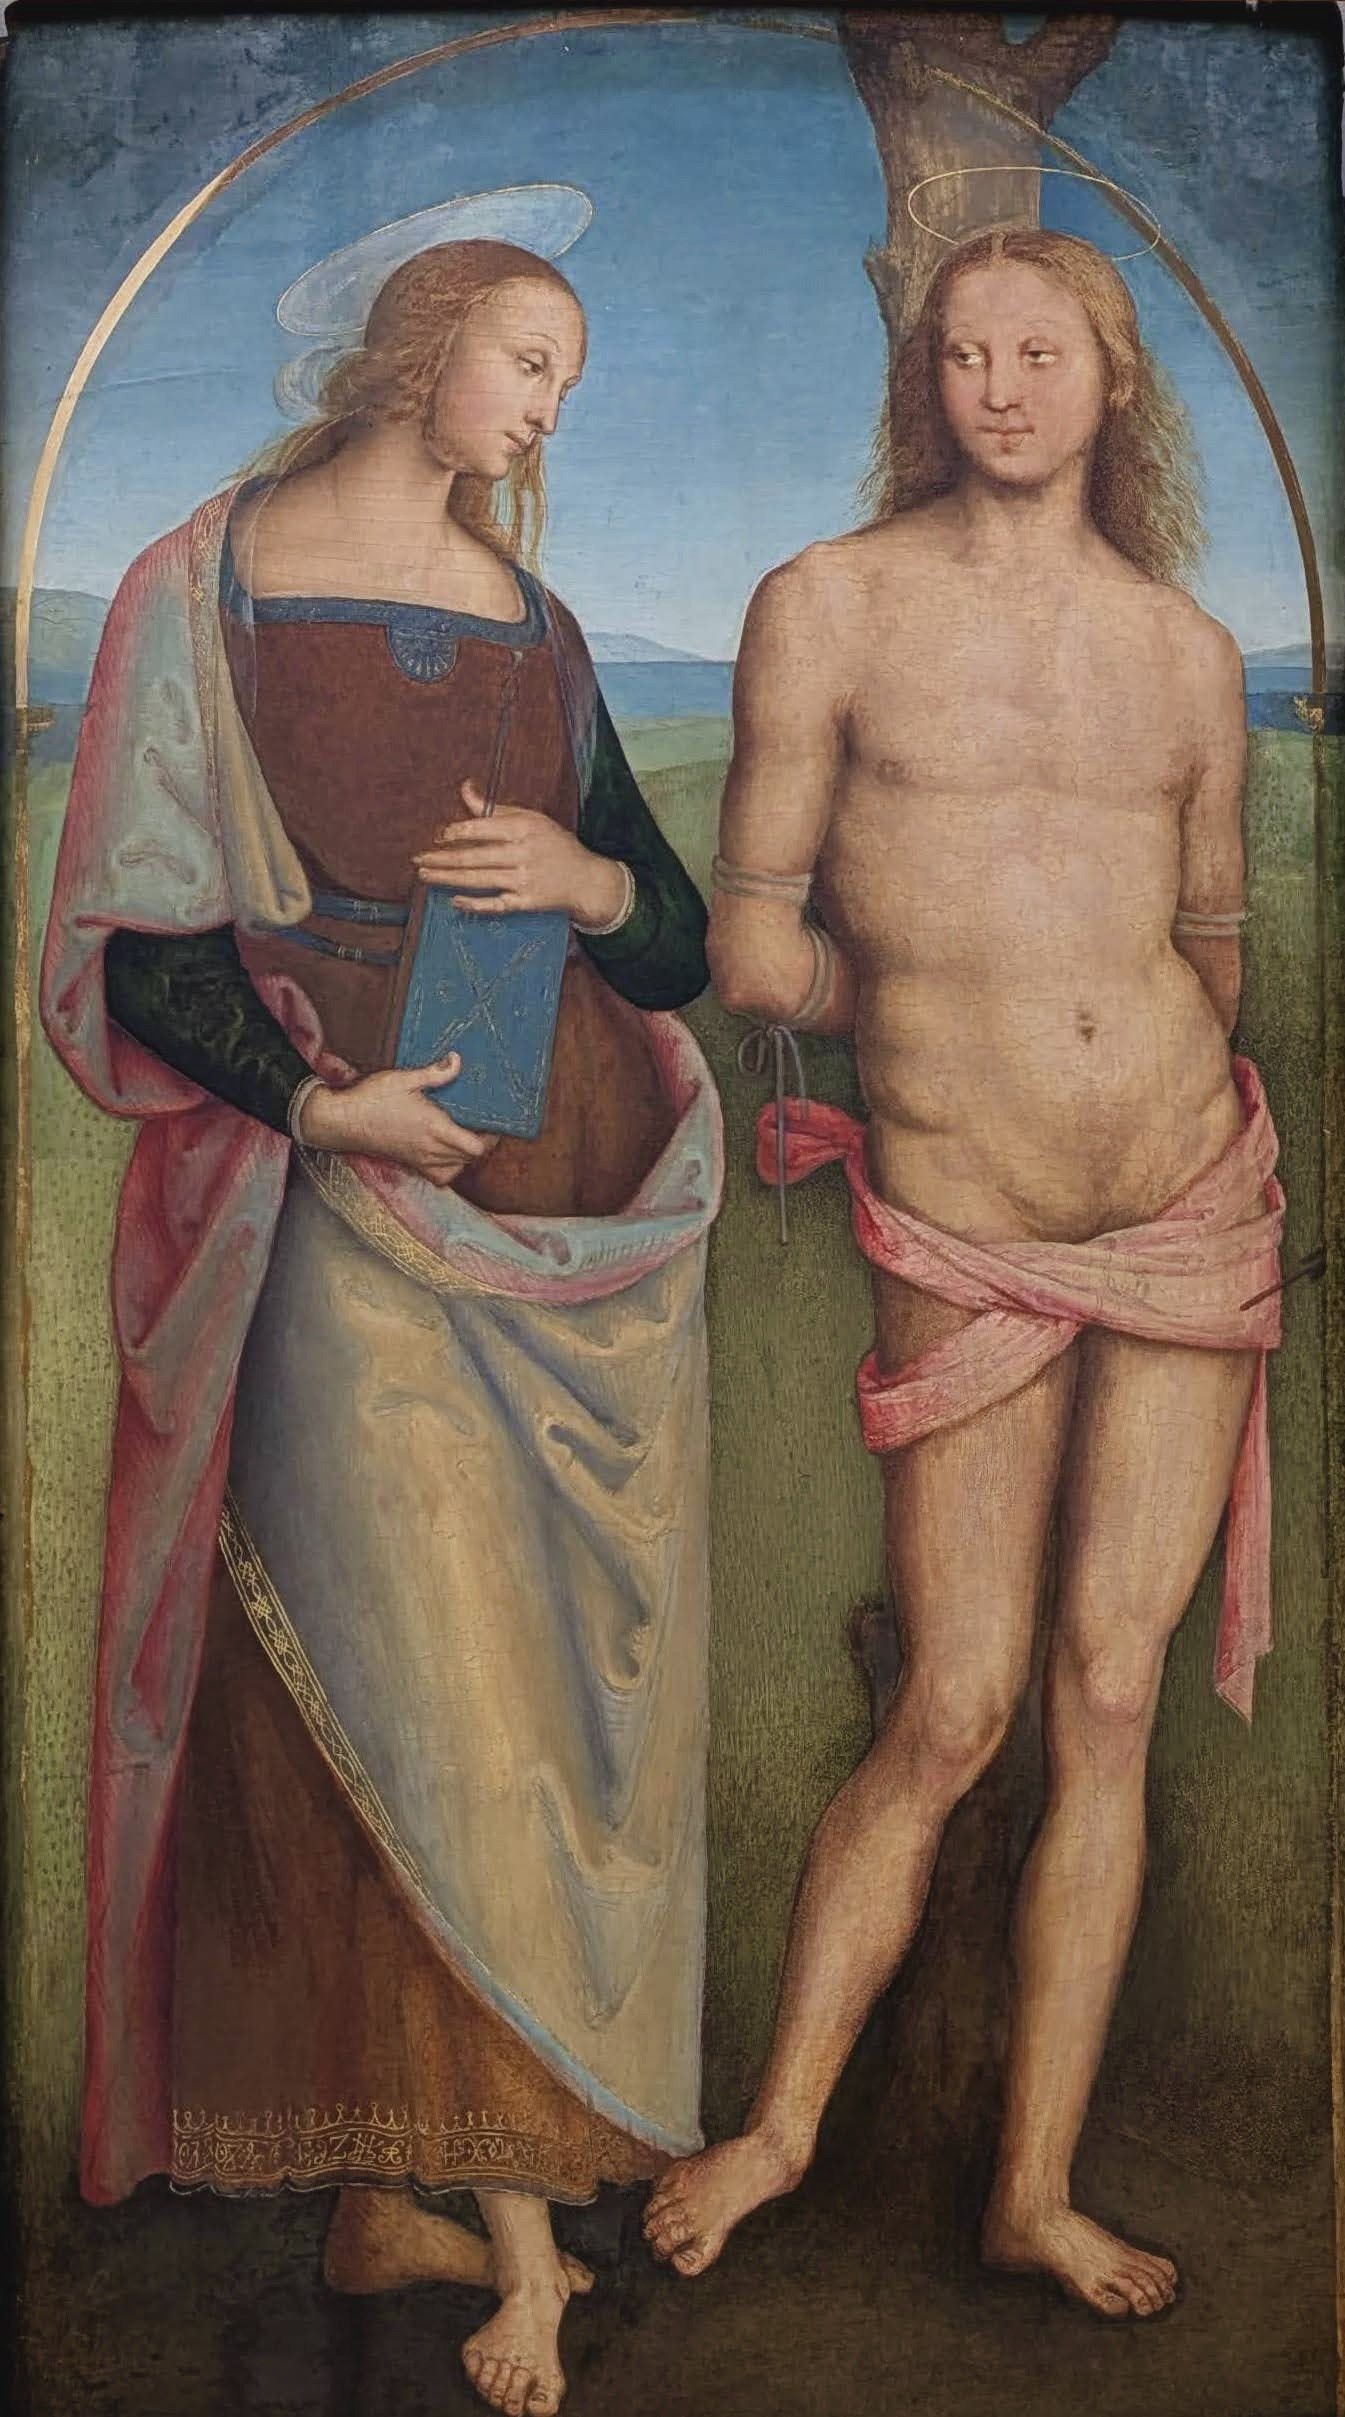
\includegraphics[height=0.4\textheight]{annexes/figures/ptrPeruginSaints.jpg}
    \caption{Pérugin, \textit{Saint Sébastien et sainte Apolline}, 1513 -1523, peinture à l'huile sur toile, Grenoble, Musée de Grenoble, inv. MG 48}
    \label{fig:ptrPeruginSaints}
\end{figure}

\begin{figure}[H]
    \centering
    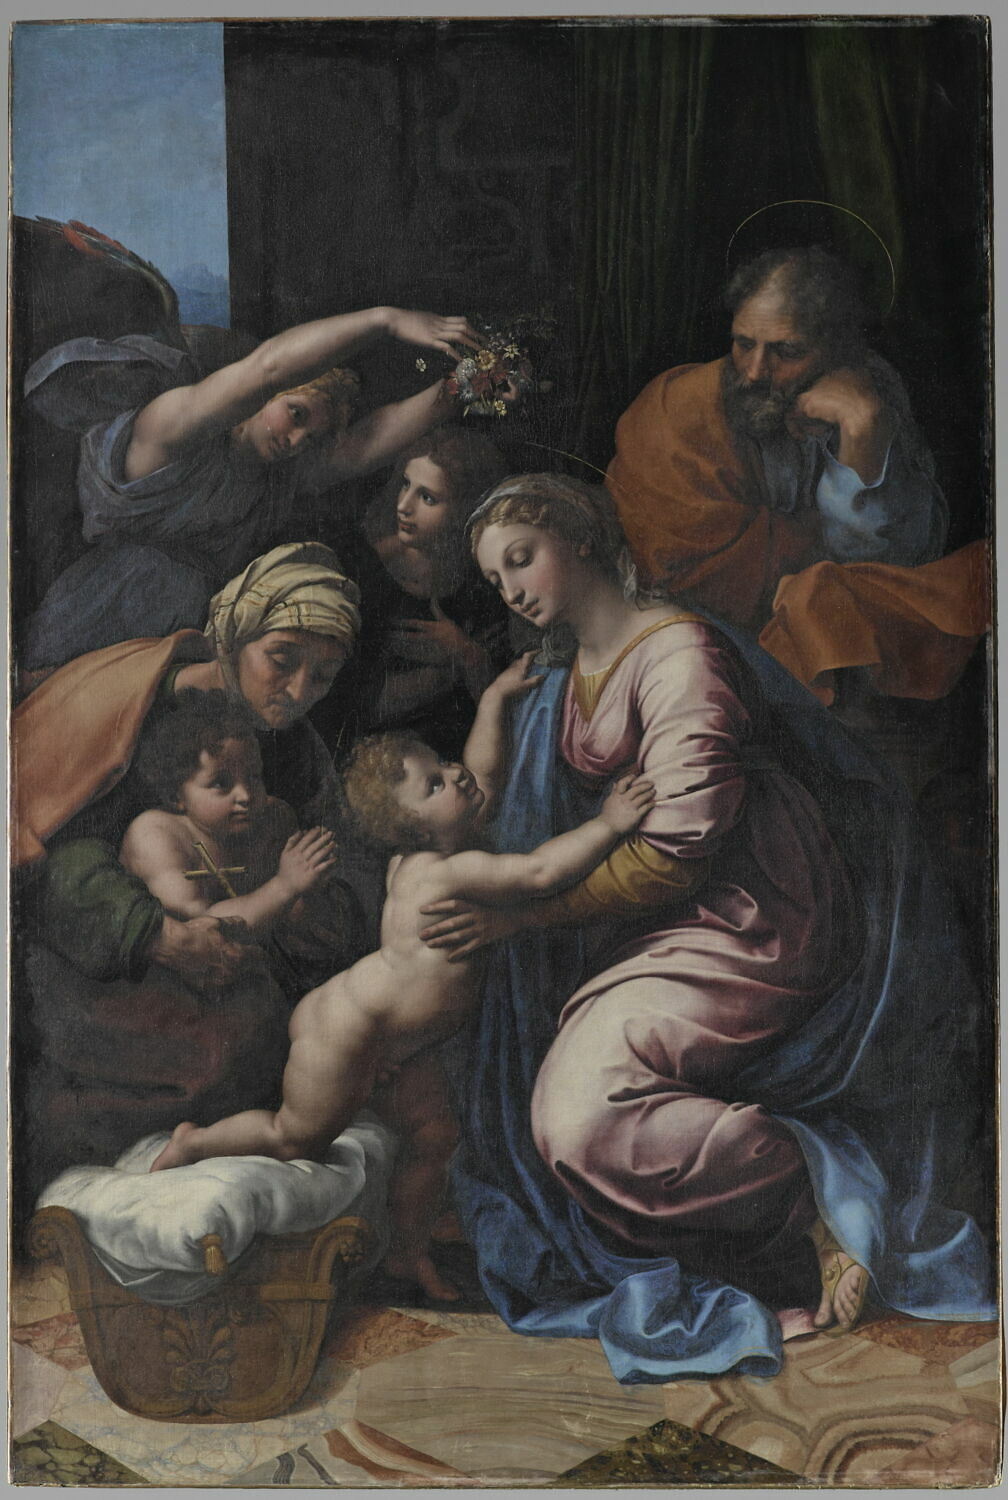
\includegraphics[height=0.4\textheight]{annexes/figures/ptrRaphaelSteFam.jpg}
    \caption{Raphaël, \textit{La Sainte Famille, dit La Grande Sainte Famille de François Ier}, 1518, peinture à l'huile sur toile, Paris, Musée du Louvre, INV 604 ; MR 432 © 2013 GrandPalaisRmn (musée du Louvre) / Adrien Didierjean}
    \label{fig:ptrRaphaelSteFam}
\end{figure}


\section{Exemples d'images inexploitables}

\begin{figure}[H]
    \centering
    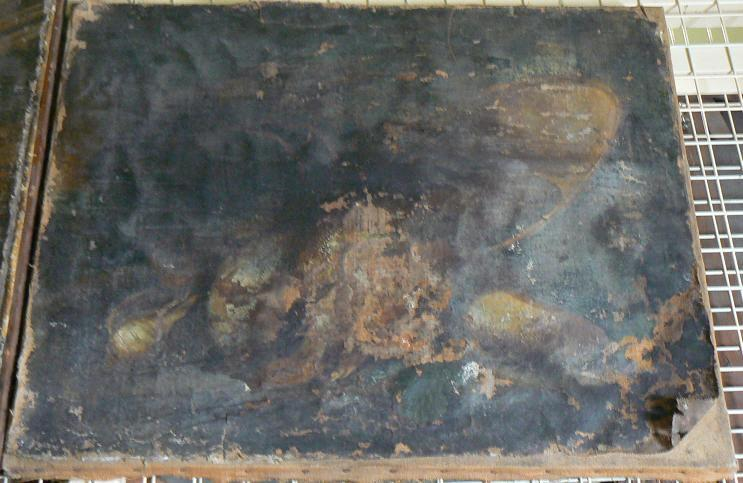
\includegraphics[height=0.4\textheight]{annexes/figures/ptrRecco.jpg}
    \caption{Raphaël, \textit{Giuseppe Recco \textit{Nature morte : poisson de mer et chaudron}, Musée des Beaux-Arts (Orléans), inv. 1173, Lien AGORHA : \\ \url{https://agorha.inha.fr/ark:/54721/d5fc162e-48a3-4508-9a6c-562fb76c1a1a}}
    \label{fig:ptrRecco}
\end{figure}

\section{L'étude comparatives des modèles}

\begin{figure}[H]
    \centering
    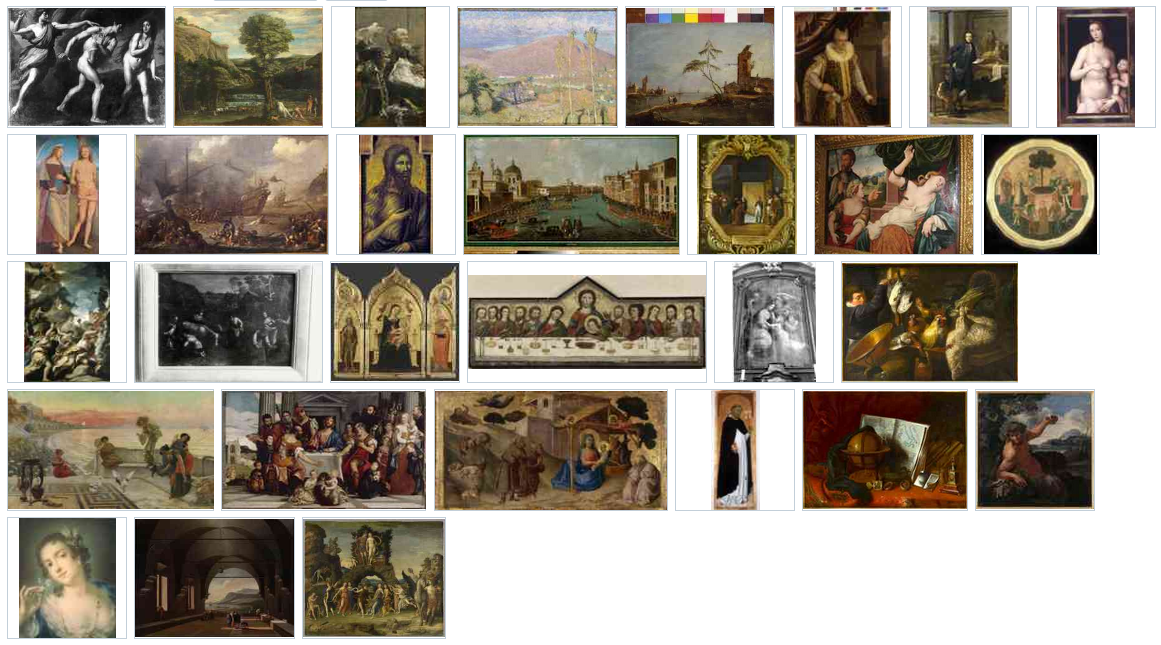
\includegraphics[width=1\textwidth]{annexes/figures/benchmark.png}
    \caption{Les trente tableaux choisis dans le Retif pour constituer le benchmark des modèles de vision par ordinateur.}
    \label{fig:benchmark}
\end{figure}

\section[Liste des peintures]{Liste des peintures utilisées pour l'étude des modèles (Chapitre 6)}
\begin{itemize}
\small
    \item Grifo di Tancredi, \textit{Saint Jean-Baptiste}, 1e quart du XIVe siècle, Musée des Beaux-Arts (Chambéry), inv. M 933. Lien AGORHA : \\ \url{https://agorha.inha.fr/ark:/54721/d72206a7-27c0-4260-8f16-dbf6fbcceab3}
    \item Maestro della Maddalena, \textit{La Cène}, 3e quart du XIIIe siècle, dépôt du musée du Louvre (Paris) au musée du Petit Palais (Avignon), inv. 1089.1. Lien AGORHA : \\ \url{https://agorha.inha.fr/ark:/54721/b5efecda-e688-41c0-a8cb-31fcde24e9b6}
    \item Andrea da Firenze, \textit{La Fontaine d'amour}, XIVe siècle, Douai, Musée de la Chartreuse, Inv. 1089. Lien AGORHA : \\ \url{https://agorha.inha.fr/ark:/54721/e5b631b2-a483-4171-bdf9-da6bfdba1115}
    \item Taddeo Gaddi, \textit{L'Adoration des bergers}, vers 1330, Dijon, Musée des Beaux-Arts, inv. 1470. Lien AGORHA : \\ \url{https://agorha.inha.fr/ark:/54721/f39e3826-f862-4489-b979-4c8063b9950b}
    \item Bartolo di Fredi, \textit{Saint Dominique}, 1397, Musée des Beaux-Arts (Chambéry), inv. D.81.1.3. Lien AGORHA : \\ \url{https://agorha.inha.fr/ark:/54721/7e0aada6-931f-4b4b-b9bc-ef0461daf983}
    \item Andrea Mantegna, \textit{Mars et Vénus}, 1496-1497, Département des peintures du musée du Louvre (Paris), INV 370. Lien AGORHA : \\ \url{https://agorha.inha.fr/ark:/54721/687cce0f-9a9e-4e3d-a826-702cf81be157}
    \item Francesco Francia, \textit{Vénus et Cupidon}, vers 1500, Musée des Beaux-Arts (Mulhouse), inv. 61.1.13. Lien AGORHA : \\ \url{https://agorha.inha.fr/ark:/54721/823a7d31-05ba-4545-81f1-b63a9b81f1b0}
    \item Le Pérugin, \textit{Saint Sébastien et sainte Apolline}, 1er quart du XVIe siècle, Musée de Grenoble, inv. MG.48.  Lien AGORHA : \\ \url{https://agorha.inha.fr/ark:/54721/ec5f09f4-6f00-457b-ba37-feaf4d63acbe}
    \item Paolo Véronèse, \textit{Les Pèlerins d'Emmaüs}, vers 1559, Musée du Louvre (Paris), inv. INV 146. Lien AGORHA : \\ \url{https://agorha.inha.fr/ark:/54721/837ec2ef-7d88-45c5-9da1-32d9860c7a28}
    \item Attribué à Francesco Montemezzano, \textit{Portrait d'une dame tenant un luth}, XVIe siècle, Musée de Picardie (Amiens), inv. MP.Lav.1894.223. Lien AGORHA : \\ \url{https://agorha.inha.fr/ark:/54721/c306700a-1c71-424e-a136-32f7f7026739}
    \item Copie anonyme d'après Jacopo Bassano, \textit{L'Automne}, XVIIe siècle, Musée Garinet (Châlons-en-Champagne), inv. 899.11.237 Lien AGORHA : \\ \url{https://agorha.inha.fr/ark:/54721/a793bae2-1995-487e-b06e-e081a94927fd}
    \item Girolamo Marchesi, \textit{La Mort de Cléopâtre}, milieu du XVIe siècle, Musée Baron Gérard (Bayeux), inv. P.0177. Lien AGORHA : \\ \url{https://agorha.inha.fr/ark:/54721/cc06cbe1-9bb2-4694-9084-4eb4ea861fe9}
    \item Ciro Ferri, \textit{Faune au verre de vin. L'Automne (?)}, XVIIe siècle, Palais Fesch-musée des beaux-arts (Ajaccio), inv. MFA 852.1.81. Lien AGORHA : \\ \url{https://agorha.inha.fr/ark:/54721/dac0ec32-4208-41dc-a22d-4bed21591c55}
    \item Entourage de Viviano Codazzi, \textit{Galerie voûtée avec un fond de marine}, milieu du XVIIe siècle, Musée des Beaux-Arts (Marseille), inv. 380. Lien AGORHA : \\ \url{https://agorha.inha.fr/ark:/54721/0dad77b7-bbee-4f1e-b33a-c96cb10203af}
    \item Giacomo Legi, \textit{Jeune homme dans un garde manger (nature morte avec gibier, volaille et mouton)}, 1e moitié du XVIIe siècle, Musée des Beaux-Arts (Bordeaux), inv. M.6243. Lien AGORHA : \\ \url{https://agorha.inha.fr/ark:/54721/50b22315-55a9-4a46-a5fc-051fd30be318}
    \item Attribué à Benedetto Fioravanti, \textit{Nature morte avec globe terrestre et carte d'Italie}, XVIIe siècle, Palais Fesch-musée des beaux-arts (Ajaccio), inv. MFA 852.1.592. Lien AGORHA : \\ \url{https://agorha.inha.fr/ark:/54721/525f10ac-19b1-44ca-8f4c-12952f913b6b}
    \item Le Dominiquin, \textit{Paysage avec Hercule combattant Acheloüs changé en taureau}, 1621-1622, Musée du Louvre (Paris), inv. INV 794. Lien AGORHA : \\ \url{https://agorha.inha.fr/ark:/54721/d629c1a1-4cd9-406c-834b-393f93d9bc24}
    \item Atelier de Luca Giordano, \textit{La Mort d'Orphée}, XVIIe siècle, Musée Hyacinthe Rigaud (Perpignan), inv. 840.2.7. Lien AGORHA : \\ \url{https://agorha.inha.fr/ark:/54721/709a2a40-0b00-4d85-b1bd-4cac2d58d31f}
    \item Ottavio Vannini, \textit{Adam et Eve chassés du Paradis terrestre}, XVIIe siècle, Musée des beaux-arts Jules Chéret (Nice), inv. 1884. Lien AGORHA : \\ \url{https://agorha.inha.fr/ark:/54721/de6f3938-90a3-4798-b0af-dcf9d2c85bf8}
    \item Cornelis de Wael, \textit{Combat naval}, XVIIe siècle, Musée d'Art et d'Histoire (Cognac), inv. 892.1.24. Lien AGORHA : \\ \url{https://agorha.inha.fr/ark:/54721/9d64e054-0e1b-45c1-ba04-35765ea39e86}
    \item Attribué à Francesco Guardi, \textit{Paysage avec marine et tours}, XVIIIe siècle, Musée de Picardie (Amiens), inv. MP.Lav.1894.217. Lien AGORHA : \\ \url{https://agorha.inha.fr/ark:/54721/e57b34cb-b772-4014-b639-ad661df64bb4}
    \item Attribué à Rosalba Carriera, \textit{L'Été}, XVIIIe siècle, Fondation Bemberg (Toulouse), inv. 1064. Lien AGORHA : \\ \url{https://agorha.inha.fr/ark:/54721/88c8ac54-99e4-4d6a-98f9-bef4d2553784}
    \item Pompeo Batoni, \textit{Portrait de Charles John Crowle (1738-1811)}, 1761-1762, Musée du Louvre (Paris), inv. RF 1981 37. Lien AGORHA : \\ \url{https://agorha.inha.fr/ark:/54721/652d90b7-46f0-406b-b34c-7c971ec44391}
    \item Luca Carlevarijs, \textit{Venise, fête sur le grand canal}, 1e moitié du XVIIIe siècle, Musée de la Castre (Cannes), inv. 35. Pe. Lien AGORHA : \\ \url{https://agorha.inha.fr/ark:/54721/cd495a47-ef36-4184-b91b-d56ddf610909}
    \item Antonio Mancini, \textit{L'Homme au perroquet}, avant 1917, Musée d'Orsay (Paris), inv. RF 1980 137. Lien AGORHA : \\ \url{https://agorha.inha.fr/ark:/54721/26e71710-c577-473b-a0eb-88e1d9734462}
    \item Luigi Rubio, \textit{Napoléon reçoit Mohammed Mirza Reza Khan, ambassadeur de Perse, à Firkenstein, 27 avril 1807}, 1834, Musée national des châteaux de Versailles et de Trianon (Versailles), inv. 1850.1442. Lien AGORHA : \\ \url{https://agorha.inha.fr/ark:/54721/b1f66158-0117-4c85-a6be-da8b69d935c8}
    \item Emilio Vasarri, \textit{Les Oies}, vers 1908, Musée d'arts de Nantes, inv. 1208. Lien AGORHA : \\ \url{https://agorha.inha.fr/ark:/54721/1f51a542-129b-45c6-897a-b94916541bca}
    \item Serafino Macchiati, \textit{Heure automnale ou L'Automne}, 1914, Musée d'Orsay (Paris) inv. INV 20241. Lien AGORHA : \\ \url{https://agorha.inha.fr/ark:/54721/8229d01a-857d-4068-8e68-de929b02eff3}
    \item Attribué à Lorenzo Vecchietta, \textit{Triptyque : La Vierge et l'Enfant couronnée par deux anges (partie centrale) ; Saint Jean-Baptiste (volet gauche) ; L'Ange de l'Annonciation (au-dessus) ; Saint Jérôme (volet droit) ; La Vierge de l'Annonciation (au-dessus)}, XVe siècle, Musée du Petit Palais (Avignon), inv.Cl. 7492. Lien AGORHA : \\ \url{https://agorha.inha.fr/ark:/54721/6730de2b-0efc-417f-8ece-7321f7ad4d28}
    \item Copie anonyme d'après Raphaël, \textit{La Grande Sainte Famille de François Ier}, début 18e siècle, Eglise Saint-Pierre (Méhoncourt). Lien AGORHA : \\ \url{https://agorha.inha.fr/ark:/54721/cdeeb0cb-ac77-4012-80bf-128fe93d0765}
\end{itemize}


